\documentclass{article}
\usepackage[letterpaper, portrait, margin=1.0in]{geometry}
\usepackage{graphicx}
\graphicspath{ {./} }


\title{CMSC 471 - Project 2}
\date{2016-03-17}
\author{Jerson Guansing}

\begin{document}
  \pagenumbering{gobble}
  \maketitle
  \newpage
  \tableofcontents
  \newpage
  \pagenumbering{arabic}

  \section{Overview}
  
  Find the global min of this function using all three of the methods you wrote above:\\
  
  $z = \frac{sin(x^2 + 3y^2)}{0.1 + r^2} + (x^2 + 5y^2) * \frac{exp(1 - r^2)}{2}, r = \sqrt{x^2 + y^2}$ \\
  
  Write a report in LaTex explaining which did better, which took longer, and why you think it is.  Use PyPlot to generate a graph of the function and see if you can graph the path your algorithm took.  You should be going from (2.5, 2.5) to (-2.5, -2.5).\\
  
  \section{Result}
  
   \subsection{Optimization Result}
  \begin{table}[h]
  	\centering
  	\caption{Optimization Result}
  	\label{tab:table1}
  	\begin{tabular}{|c|c|c|c|c|}
  	\hline
  	Method & Total Plots & x & y & z \\
  	\hline
  	hill climbing & 83 & 0.0019 & -0.0045 & 0.0066 \\
  	\hline
  	hill climbing with random restart & 1027 & -2.1718 & -0.0011 & -0.1542 \\
  	\hline
  	simulated annealing & 57 & -2.0989 & -0.3323 & -0.1472 \\
  	\hline
  \end{tabular}
  \end{table}
  
  \subsection{Which did better}
  Of the three methods, hill climbing with random restart got the best results (smallest min value), and then followed by simulated annealing and then hill climbing. In all the test trials, hill climbing with random restart managed to overcome the main issue of getting stuck on local minima with a relatively small number of restarts (10). However, the result is still highly dependent on the number of undulation within the function, and the likelihood that a random restart will lead to a neighboring path of the global minimum. This is the very same reason why hill climbing did the worst of the three methods due to the lack of recourse to overcome local minima. On the other hand, simulated annealing minimizes the function by picking a random move instead of the best neighbor, and then checking if it improves the situation (if not, the algorithm accepts the new value with some probability $e^\frac{-\Delta E}{T} < 1$).\\
 
 \subsection{Which took longer}
 However, hill climbing with random restart took the longest of the three methods as it has the largest scatter plot size. It was able to get the best result of the three methods because the algorithm searched through more nodes (from the random starting point up to the neighboring path minima; repeat N number of times). Similarly, hill climbing uses the same approach (without the random restart) as it examines all the neighboring nodes until it find the path's local minima (smaller possibility to be the global minima for functions with higher number of undulation). In contrast, simulated annealing converges quickly which results in smaller scatter plot size and faster algorithm. The algorithm checks $\Delta E$ and the random move's probability which is exponentially decreases with the badness of moves. Hill climbing only received faster runtime when the starting random value are located close to a local minima.
  
  \newpage
  
 \section{Graphs}
 
 \subsection{Hill Climbing Graph}
 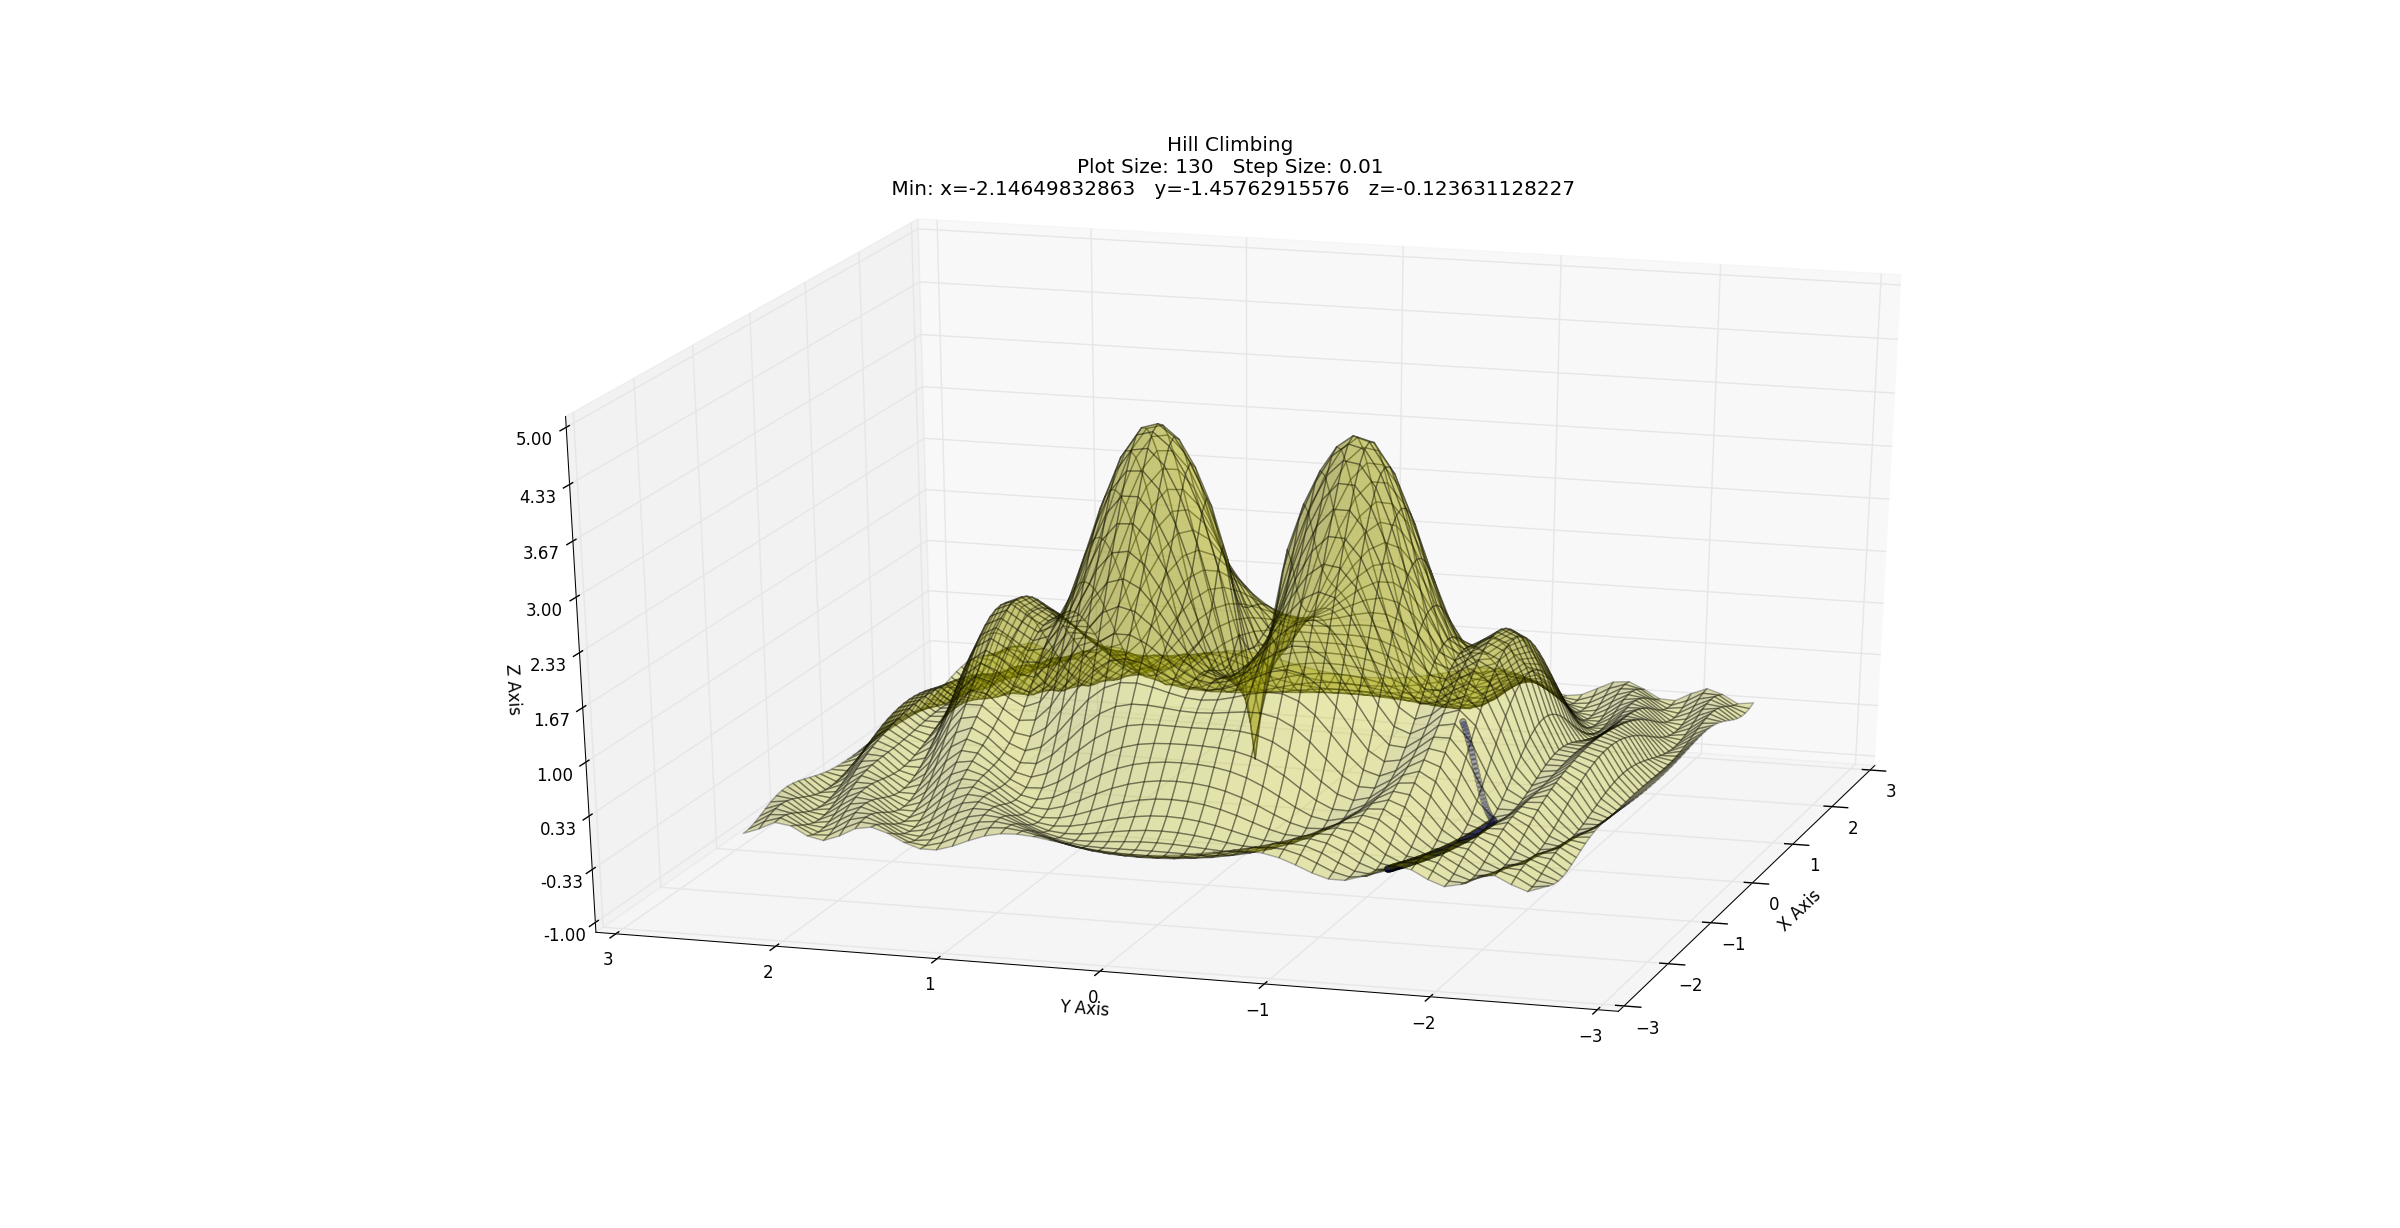
\includegraphics[width=1.1\textwidth]{figure_1h.png}
	
	hill climb(function to optimize, step size, xmin, xmax, ymin, ymax):\\
	step size = 0.01, xmin = -2.5, xmax = 2.5, ymin = -2.5, ymax = 2.5\\
		
	This function randomly picks a starting point, and then runs the hill climbing algorithm. Since the goal is to minimize the function,it will only look for values lower than the current node, and will end the search if all the neighbors have a higher value. This means that the minimum value returned might be a local minimum which is the case displayed in this graph.\\

 
 \subsection{Hill Climbing with Random Restart Graph}
 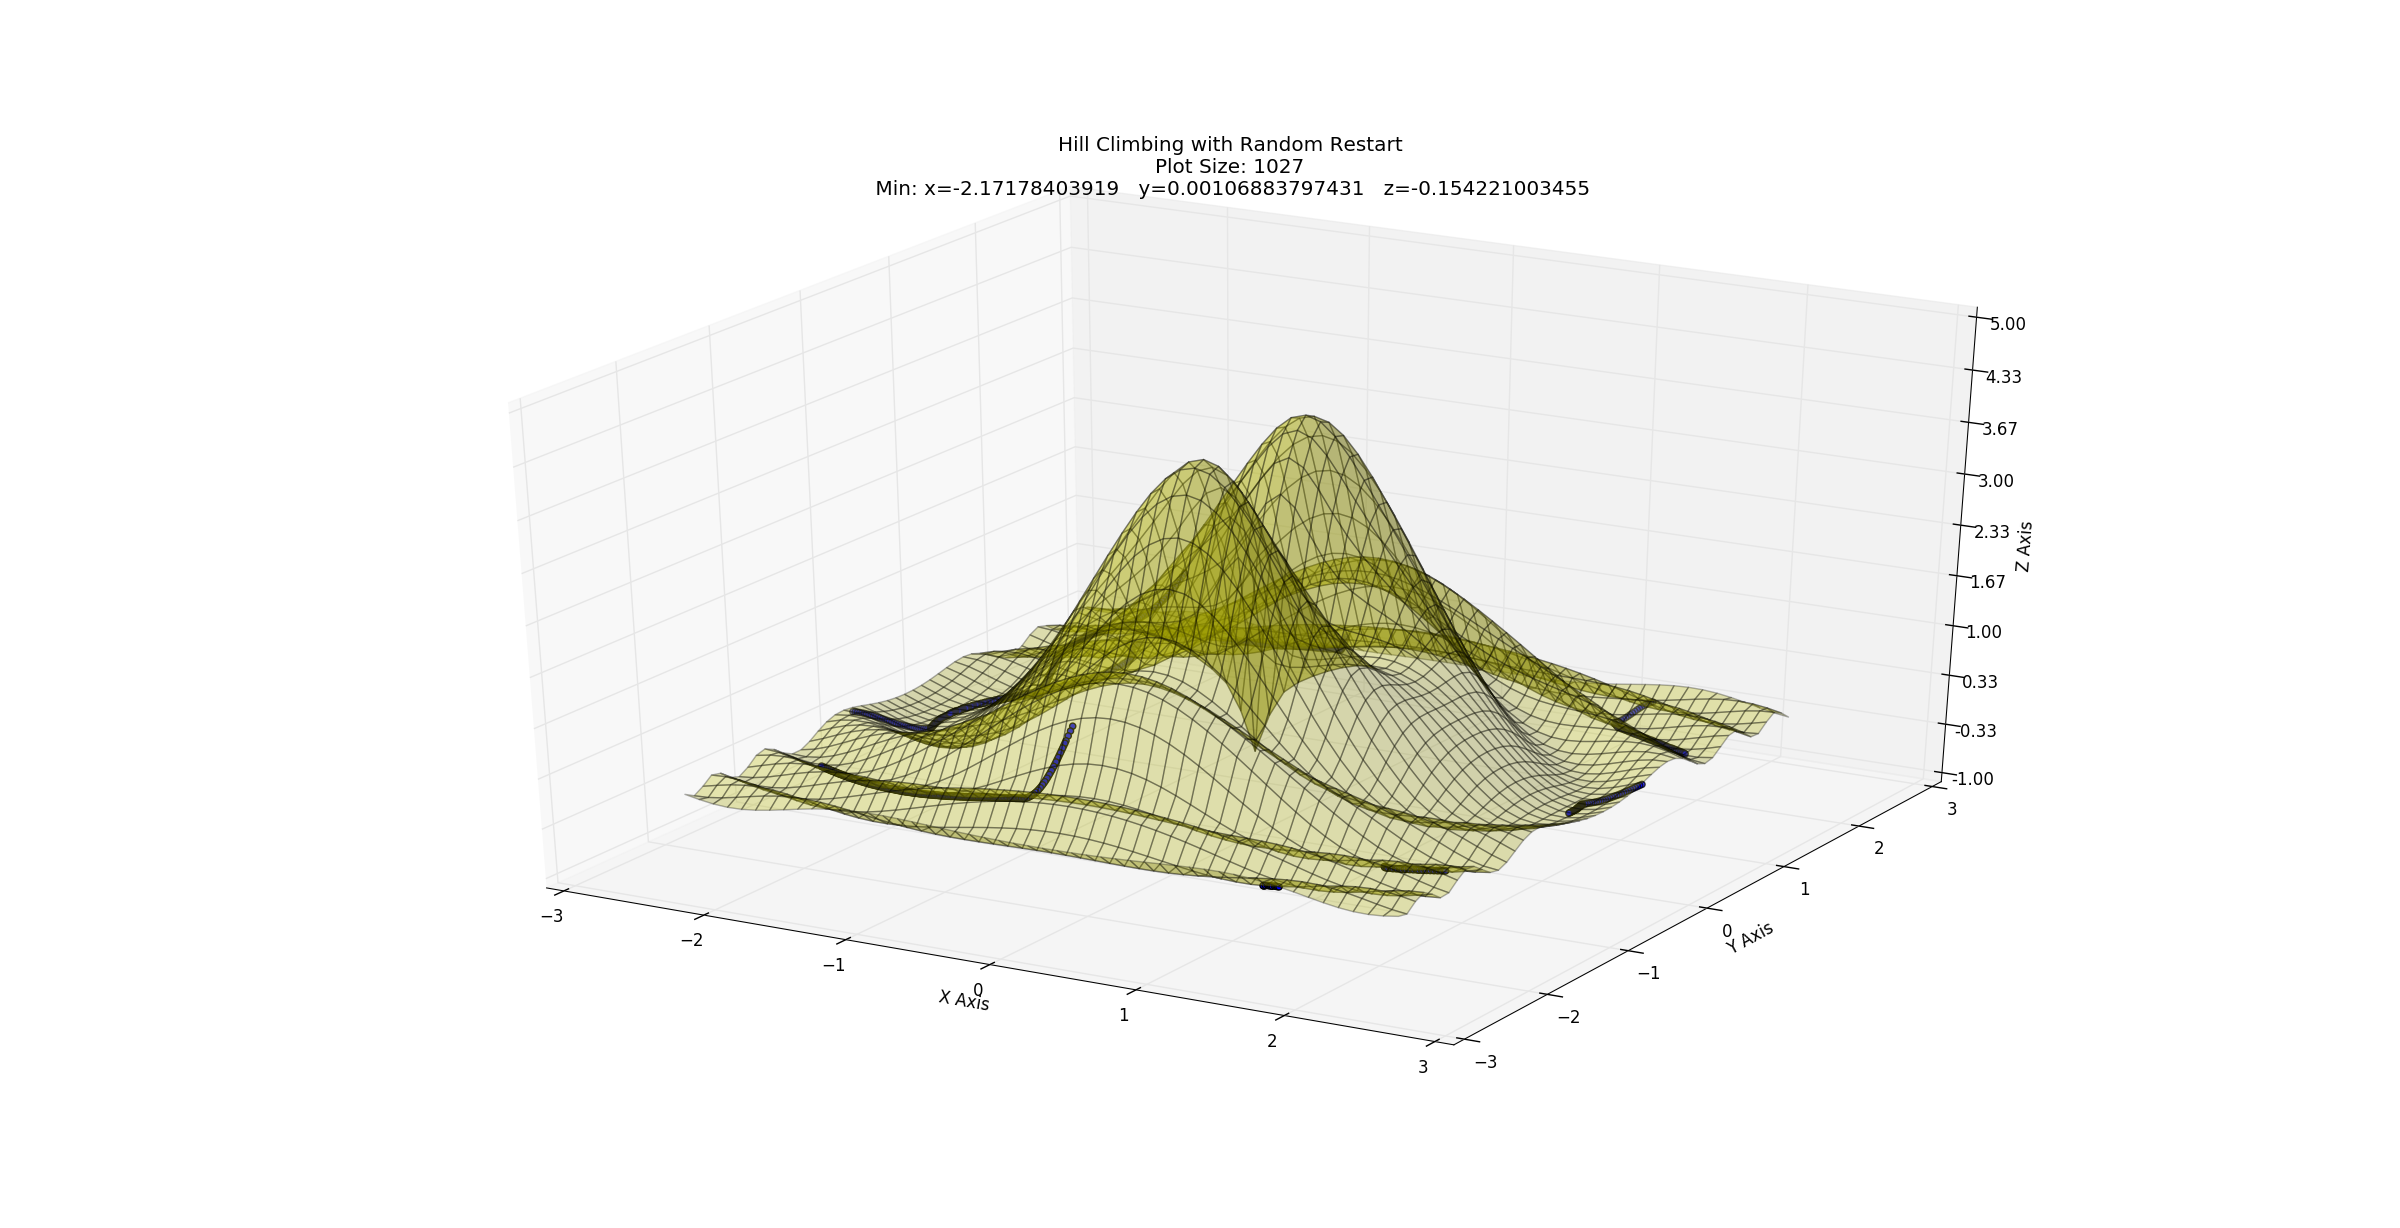
\includegraphics[width=1.1\textwidth]{figure_2h.png}

	hill climb random restart(function to optimize, step size, num restarts, xmin, xmax, ymin, ymax):\\
	step size = 0.01, num restarts = 10, xmin = -2.5, xmax = 2.5, ymin = -2.5, ymax = 2.5\\
	
	This function calls the hill climbing function N number of times. Each iteration returns the path list that is added to the total scatter plot, and track the best value or minimum. The random restarts allow the function to compensate for the shortcomings of the hill climbing function in exchange for longer runtime. This means that the minimum value returned is closer or has a higher chance to be the global minimum due to random samplings of the function.\\
  
  
  \subsection{Simulated Annealing Graph}
  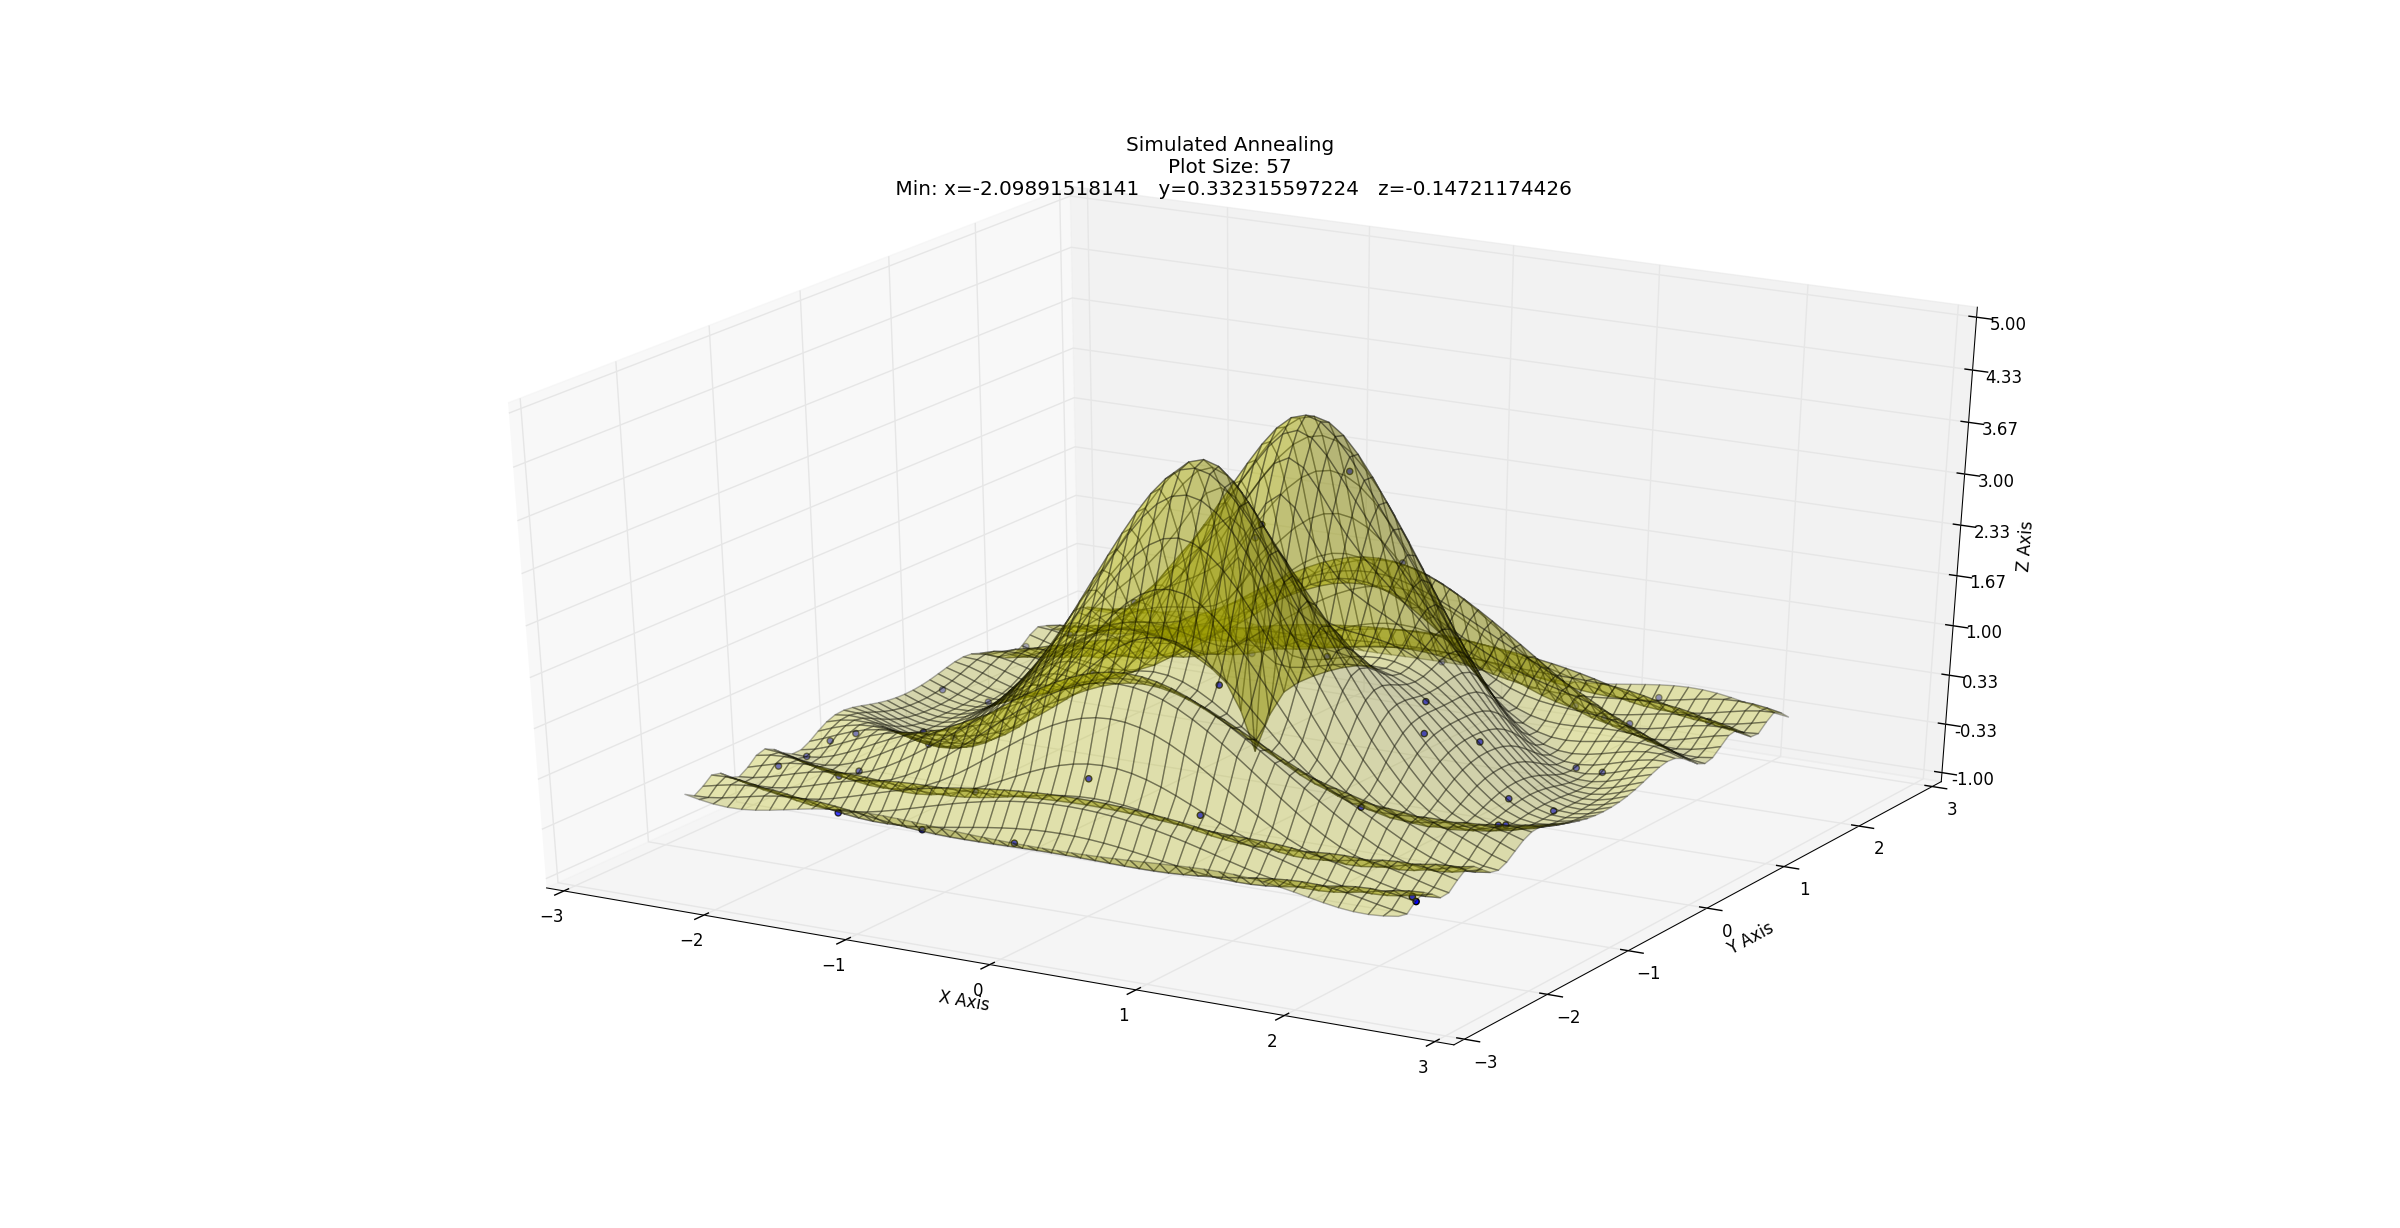
\includegraphics[width=1.1\textwidth]{figure_3h.png}
   
   simulated annealing(function to optimize, step size, max temp, xmin, xmax, ymin, ymax):\\
   step size = 0.01, max temp = 50, xmin = -2.5, xmax = 2.5, ymin = -2.5, ymax = 2.5\\
   
   Unlike hill climbing, this function picks a random move instead of the best move. If $\Delta E$ or ( f(new) - f(current)) improves the situation which in this case is ($\Delta E < 0$), then it is accepted since the new Z value is lower than the current one. Otherwise, the algorithm accepts the new value with some probability $e^\frac{-\Delta E}{T} < 1$. The probability decreases exponentially as the temperature is gradually decreased to 0. The function keeps track of the best value or the minimum as each iteration is added to the path list.
	  
\end{document}